% -*-mode: Latex-*-
% !TEX root = thesis.tex
% paper: ...
% authors: simon maurer
%
% file: ecm.tex
% contents: process network with synchronous communication
% Sccs-Id: %W% %G%
\chapter{PNSC with SIA - An Analysable Event-based Component Model}
\label{chap_ecm}

In this chapter I present a model that allows to describe the interaction of concurrent components.
Each component is modelled as a, possibly stateful, process that is interacting with its environment by reacting to input messages and producing output messages.
A process follows the sporadic communication semantics, as described in \SSect{\ref{sect_background_com}}.

The chapter is structured as follows:
\Sect{\ref{sect_ecm_pnsc}} defines the model, called \gls{pnsc}, where concurrent processes build a network by interacting over synchronous communication channels.
The synchronous communication model imposes strict blocking rules on the communication which allows to gain a deeper understanding of the interaction.
In \Sect{\ref{sect_ecm_sia}} I introduce \glspl{sia}, a model to describe the interaction protocol of processes.
It serves to describe how a process interacts with its environment and whether potential problems, such as permanent blocking situations, can occur.
In \Sect{\ref{sect_ecm_example}} I describe how the \gls{pnsc} model can be used to model an example of a traffic situation on an intersection.
Further, I extend the example by modelling an assembly of intersections as streaming network with buffered communication.
Finally, in \Sect{\ref{sect_ecm_summary}} I summarise the chapter.

%==============================================================================
\section{Process Networks with Synchronous Communication (PNSC)}
\label{sect_ecm_pnsc}
The communication model of process networks described in this chapter is based on synchronous communication.
For further reference I use the name \emph{\acrfull{pnsc}}.
A \gls{pnsc} consists of a set of processes $PN$.
A process in a \gls{pnsc} interacts with other processes via input and output ports.

\begin{definition}[PNSC Process]
    \label{def_proc}
    Formally, a process $N$ is defined as a tuple
    \begin{displaymath}
        N = \langle \mathcal{P}_N^I, \mathcal{P}_N^O \rangle
    \end{displaymath}
    where
    \begin{itemize}
        \item $\mathcal{P}_N^I$ is the finite set of input ports of process $N$.
        \item $\mathcal{P}_N^O$ is the finite set of output ports of process $N$.
        \item $\mathcal{P}_N$ is the \emph{signature} of process $N$ and is defined as: $\mathcal{P}_N = \mathcal{P}_N^I \cup \mathcal{P}_N^O$.
            The ports of these two port sets have to be mutually distinctive: \hbox{$\mathcal{P}_N^I \cap \mathcal{P}_N^O = \emptyset$}.
    \end{itemize}
\end{definition}

% Let $\mathcal{P}_N^I$ be the set of input ports of a process $N \in PN$ and $\mathcal{P}_N^O$ the set of output ports of $N$.
% The set of all ports $\mathcal{P}_N = \mathcal{P}_N^I \cup \mathcal{P}_N^O$ of a process $N$ forms the \emph{signature} of the process.
A process is of type \emph{\gls{mimo}}, hence it holds that
$$|\mathcal{P}_N^I| \geq 0 \land |\mathcal{P}_N^O| \geq 0$$
Note, that a process can have a persistent state and thus, is not necessarily functional.

Two processes $M$ and $N$ are connected through synchronous channels if they have \emph{shared} ports.
One end of the channel connects to an input port of one process and the other end connects to an output port with the same name of the other process.
The shared ports of processes $M$ and $N$ are defined in \Equ{\ref{eq_shared_ports}}.
\begin{equation}
    \label{eq_shared_ports}
    shared_{\mathcal{P}}(M, N) = \big ( \mathcal{P}_M^I \cap \mathcal{P}_N^O \big ) \cup \big (\mathcal{P}_M^O \cap \mathcal{P}_N^I \big )
\end{equation}

All ports in a set of $n$ processes $\mathit{PN} = \{N_0, \dots, N_n\}$ describing a \gls{pnsc} must be non-conflicting:
\begin{eqnarray}
    \label{eq_conflict_port_in}
    \bigcap_{i=0}^n \mathcal{P}_{N_i}^I &=& \emptyset \\
    \label{eq_conflict_port_out}
    \bigcap_{i=0}^n \mathcal{P}_{N_i}^O &=& \emptyset
\end{eqnarray}

I distinguish between two types of processes, an \emph{atomic process} and a \emph{composed process}.
An atomic process is a black box where the implementation of the process is unknown to the model.
A composed process is an abstraction of a \gls{pnsc} in the sense that the processes of the \gls{pnsc} are composed into a single process.
The signature of a composed process is formed out of non-connected ports of each process in the set of the \gls{pnsc} abstracted by the composed process as defined by \Def{\ref{def_proc_composed}}.
This composition can be applied incrementally on a set of processes in any order if \Equ{\ref{eq_conflict_port_in}} and \Equ{\ref{eq_conflict_port_out}} are satisfied.

\begin{definition}[Composed PNSC Process]
    \label{def_proc_composed}
    Let ${M, N}$ be the set of processes of a \gls{pnsc}.
    Formally, the signature $\mathcal{P}_{\mathit{MN}}$ of the composed process $\mathit{MN}$ is defined as follows:
    \begin{displaymath}
        \mathcal{P}_{\mathit{MN}}^I = (\mathcal{P}_M^I \cup \mathcal{P}_N^I) \setminus shared_\mathcal{P}(M, N)
    \end{displaymath}
    \begin{displaymath}
        \mathcal{P}_{\mathit{MN}}^O = (\mathcal{P}^O_M \cup \mathcal{P}_N^O) \setminus shared_\mathcal{P}(M, N)
    \end{displaymath}
\end{definition}

\Fig{\ref{fig_cross_proc_dl}} depicts the process model of the crossroad example introduced in \Sect{\ref{sect_background_comp}}.
The four processes $P_{\mathit{NW}}$, $P_{\mathit{NE}}$, $P_{\mathit{SE}}$, and $P_{\mathit{SW}}$ in \Fig{\ref{fig_cross_proc_atomic}} represent the guards for the mutually exclusive allocation of the four critical sections $\mathit{NW}$, $\mathit{NE}$, $\mathit{SE}$, and $\mathit{SW}$.
Processing the messages $m_{wi}$, $m_{ni}$, $m_{ei}$, and $m_{si}$ represent the advancing of a car from the corresponding direction onto the respective spaces $\mathit{NW}$, $\mathit{NE}$, $\mathit{SE}$, and $\mathit{SW}$.
Similarly, processing the messages $m_{w}$, $m_{n}$, $m_{e}$, and $m_{s}$ represent the advancing of a respective car by one space: $\mathit{NW} \rightarrow \mathit{NE}$, $\mathit{NE} \rightarrow \mathit{SW}$, $\mathit{SE} \rightarrow \mathit{SW}$, and $\mathit{SW} \rightarrow \mathit{NW}$.
Producing the messages $m_{wo}$, $m_{no}$, $m_{eo}$, and $m_{so}$ represents freeing the respective spaces $(\mathit{NW}, \mathit{NE})$, $(\mathit{NE}, \mathit{SE})$, $(\mathit{SE}, \mathit{SW})$, and $(\mathit{SW}, \mathit{NW} )$.
%------------------------------------------------------------------
\begin{figure}[bht]
    \TopFigSpace
    \centering
    \begin{subfigure}[t]{0.56\textwidth}
        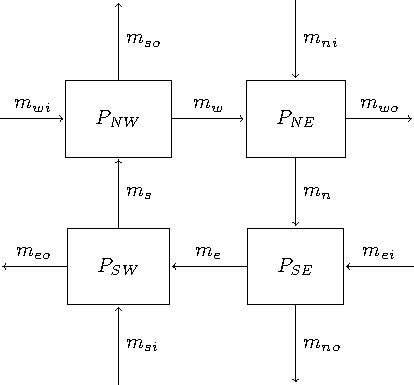
\includegraphics[width=\textwidth]{fig/cross_proc_dl.pdf}
        \CaptionFigSpace
        \caption{The \gls{pnsc} network of atomic processes.}
        \label{fig_cross_proc_atomic}
    \end{subfigure}
    ~~
    \begin{subfigure}[t]{0.34\textwidth}
        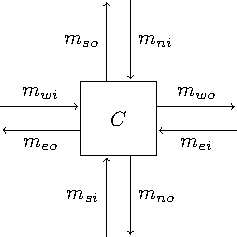
\includegraphics[width=\textwidth]{fig/cross_proc_composed.pdf}
        \CaptionFigSpace
        \caption{The \gls{pnsc} network as composed process where pairs of atomic processes are composed incrementally.}
        \label{fig_cross_proc_composed}
    \end{subfigure}
    \caption{The \gls{pnsc} network modelling the crossroad example depicted in \Fig{\ref{fig_cross_sync}}.}
    \label{fig_cross_proc_dl}
    \BotFigSpace
\end{figure}
%------------------------------------------------------------------

Due to the synchronous communication semantics of \glspl{pnsc}, in order to communicate a message from one process to another, both, the sender and receiver process must be ready at the same time for the transaction.
As processes in \glspl{pnsc} can be stateful, in order for a process to be able to send a message, the receiver process must be in a state where it is ready to receive the message.
Otherwise, the sending process is temporarily blocking in its current send state.
Similarly, for a process to be able to receive a message, the sending process must be in a state where it is able to send the message.
Otherwise, the receiving process is temporarily blocking in its current receive state.
% If a process $N$ is not in the corresponding state to perform the necessary action required by a process $M$, process $M$ is temporarily blocking and waits for process $N$ to reach the state where it is ready to perform the message transmission.

If a process resides in a blocking state indefinitely, the \gls{pnsc} (or a subset of the processes in the \gls{pnsc}) is in a permanent blocking state.
The question that arises is how to detect such permanent blocking states and how to decide if a \gls{pnsc} is free of any possibility to enter a permanent blocking state.
To answer this question I first need to describe the abstract behaviour of processes in order to understand how they interact with each other.
To do this I introduce \acrfullpl{sia} in the next section.

%==============================================================================
\section{Synchronous Interface Automata (SIA)}
\label{sect_ecm_sia}

A \emph{\acrfull{sia}} $\descSIA{N}$ is a finite state automaton that describes the interaction protocol of a process $N$ with its environment.

%------------------------------------------------------------------------------
\subsection{Definition of SIAs}
The alphabet of a \gls{sia} is a set of \emph{actions} where each action describes the label of a transition from one protocol state to another.
% The alphabet of a \gls{sia} is limited to the namespace spanned by the set of ports $\mathcal{P}_N$ of process $N$ (see \Sect{\ref{sect_sia_proc}}).
The states of a \gls{sia} $\descSIA{N}$ do not necessarily represent the internal states of a process $N$ but only the states of the interaction protocol of process $N$.

\begin{definition}[SIA]
    \label{def_sia}
    Formally, a \acrfull{sia} $\descSIA{N}$ of a process $N$ (defined in \Def{\ref{def_proc}}) is defined as a tuple
    \begin{displaymath}
        \descSIA{N} = \langle S_{\descSIA{N}}, s_{\descSIA{N}}, \mathcal{A}_{\descSIA{N}}^I, \mathcal{A}_{\descSIA{N}}^O, \mathcal{A}_{\descSIA{N}}^H, \delta_{\descSIA{N}} \rangle
    \end{displaymath}
    where
    \begin{itemize}
        \item $S_{\descSIA{N}}$ is the finite set of interface states of \gls{sia} $\descSIA{N}$.
        \item $s_{\descSIA{N}} \in S_{\descSIA{N}}$ is the unique initial interface state of \gls{sia} $\descSIA{N}$.
        \item $\mathcal{A}_{\descSIA{N}}^I \subseteq \mathcal{P}_N^I$ is the finite set of input actions of \gls{sia} $\descSIA{N}$.
        \item $\mathcal{A}_{\descSIA{N}}^O \subseteq \mathcal{P}_N^O$ is the finite set of output actions of \gls{sia} $\descSIA{N}$.
        \item $\mathcal{A}_{\descSIA{N}}^H$ is the finite set of internal (\ie, hidden) actions of \gls{sia} $\descSIA{N}$.
        \item $\mathcal{A}_{\descSIA{N}}$ is the total finite set of actions. $\mathcal{A}_{\descSIA{N}}$ is defined as: $\mathcal{A}_{\descSIA{N}} = \mathcal{A}_{\descSIA{N}}^I \cup \mathcal{A}_{\descSIA{N}}^O \cup \mathcal{A}_{\descSIA{N}}^H$.
            The actions of these three action sets have to be mutually distinctive: \hbox{$\mathcal{A}_{\descSIA{N}}^I \cap \mathcal{A}_{\descSIA{N}}^O \cap \mathcal{A}_{\descSIA{N}}^H = \emptyset$}.
        \item $\delta_{\descSIA{N}}$ is the finite set of interface state transitions of \gls{sia} $\descSIA{N}$: $\delta_{\descSIA{N}} \subseteq S_{\descSIA{N}} \times \mathcal{A}_{\descSIA{N}} \times S_{\descSIA{N}}$.
            Note that an action $a \in \mathcal{A}_{\descSIA{N}}$ is not limited to a single state transition but can be part of multiple state transitions in \gls{sia} $\descSIA{N}$.
    \end{itemize}
\end{definition}

The actions in $\mathcal{A}^I$ and $\mathcal{A}^O$ are \emph{blocking} and \emph{non-autonomous}, while actions in $\mathcal{A}^H$ are \emph{non-blocking} and \emph{autonomous}.
The progress of {\em non-autonomous} actions depends on the environment, while the progress of {\em autonomous} actions is independent of the environment.
Hence, autonomous actions are controlled by the process while non-autonomous actions are controlled by the environment.
Blocking actions will wait until the environment provides the corresponding action, while non-blocking actions can be processed immediately.

%The blocking property describes whether the protocol is allowed to wait in a state until the environment is able to provide a corresponding communication partner.
%A non-blocking action is assumed to immediately trigger a transition from its current state, independent of external interference.
%The autonomy property describes whether an action can be influenced by another action or whether it is occurring independent of the environment.

Note that \glspl{sia} are input and output deterministic (hidden actions do not require determinism), which is formally defined as:
% \begin{displaymath}
%     \forall \langle s_i, a, s_j\rangle \in \delta,\ \nexists s_k \in S \ . \ (s_j \neq s_k)\ \land \ a \in (\mathcal{A}^I \cup \mathcal{A}^O)\ \land \ \langle s_i, a, s_k\rangle \in \delta
% \end{displaymath}
\begin{displaymath}
    \forall \langle s_i, a, s_j \rangle \in \delta \ . \ \langle s_i, a, s_k \rangle \in \delta \ . \ a \in (\mathcal{A}^I \cup \mathcal{A}^O)\ \implies s_j = s_k
\end{displaymath}
Above condition means that from one interface state any action $a \in (\mathcal{A}^I \cup \mathcal{A}^O)$ can be part of at most one outgoing transition.
An action $a \in \mathcal{A}$ is called \emph{enabled} in a state $s \in S$ if and only if the condition defined in \Equ{\ref{eq_sia_enabled}} is satisfied.
\begin{equation}
    \label{eq_sia_enabled}
    \exists s' \in S \ . \ \langle s, a, s' \rangle \in \delta
\end{equation}

It might be desirable for a protocol to reach a certain state in which it will reside indefinitely.
% In fact, all the processes in the examples depicted in Figures \ref{fig.sia.control.shared}, \ref{fig.sia.control.open}, and \ref{fig.sia.control.internal} imply such a behaviour because their corresponding \glspl{sia} have one or multiple states where no further transition is possible.
Hence, I define a set of \emph{end states} $S^{end}$ of a \gls{sia} in \Equ{\ref{eq_sia_end}}.
\begin{equation}
    \label{eq_sia_end}
    S^{end} = \Big \{ s \in S \ | \ \forall s' \in S, \forall a \in \mathcal{A} \ . \ \langle s, a, s' \rangle \notin \delta \Big \}
\end{equation}
Informally, an end state is a state where no further transition, triggered by any action, is possible.
Note that this holds for any action, \ie no distinction is made between different action types.

As two processes can share ports, their corresponding \glspl{sia} can share actions.
In fact, for two processes $M$ and $N$ to interact, their corresponding \glspl{sia} $\descSIA{M}$ and $\descSIA{N}$ must have \emph{shared} actions.
Shared actions are defined in \Equ{\ref{eq_shared_actions}} which is similar to the definition of shared ports of \Equ{\ref{eq_shared_ports}}.
\begin{equation}
    \label{eq_shared_actions}
    shared_{A}(\descSIA{M}, \descSIA{N}) = \big ( \mathcal{A}_{\descSIA{M}}^I \cap \mathcal{A}_{\descSIA{N}}^O \big ) \cup \big (\mathcal{A}_{\descSIA{M}}^O \cap \mathcal{A}_{\descSIA{N}}^I \big )
\end{equation}
From \Equ{\ref{eq_shared_ports}}, \Equ{\ref{eq_pi_ai}}, and \Equ{\ref{eq_po_ao}} it follows that $shared_{\mathcal{A}}(\descSIA{M}, \descSIA{N}) \subseteq shared_{\mathcal{P}}(M, N)$, which means that not all ports of the process interface have to be used by its \gls{sia}.
The set of actions that is excluded from the set of shared actions is called \emph{ignored} actions and is defined in \Equ{\ref{eq_ignored_actions}}.
\begin{equation}
    \label{eq_ignored_actions}
    ignored_{\mathcal{A}}(\descSIA{M}, \descSIA{N}) = shared_{\mathcal{P}}(M, N) \setminus shared_{\mathcal{A}}(\descSIA{M}, \descSIA{N})
\end{equation}

All input and output actions of the \glspl{sia} $\descSIA{M}$ and $\descSIA{N}$ that do not correspond to the set of shared ports of the processes $M$ and $N$ are called \emph{open} actions.
Open actions are defined in \Equ{\ref{eq_open_actions}}.
\begin{equation}
    \label{eq_open_actions}
    open_{\mathcal{A}}(\descSIA{M},\descSIA{N}) = \big ( \mathcal{A}_{\descSIA{M}}^I \cup \mathcal{A}_{\descSIA{N}}^I \cup \mathcal{A}_{\descSIA{M}}^O \cup \mathcal{A}_{\descSIA{N}}^O \big ) \setminus shared_{\mathcal{P}}(M, N)
\end{equation}

%------------------------------------------------------------------------------
\subsection{Composition of SIAs}
\label{sect_sia_composition}
Two \glspl{sia} $\descSIA{M}$ and $\descSIA{N}$ can be composed into a combined \gls{sia} $\descSIA{\mathit{MN}}$ if their actions are non-conflicting as defined in \Equ{\ref{eq_sia_def}}.
\begin{eqnarray}
    \label{eq_sia_def}
    \mathcal{A}_{\descSIA{M}}^I \cap \mathcal{A}_{\descSIA{N}}^I &=& \emptyset \nonumber \\
    \mathcal{A}_{\descSIA{M}}^O \cap \mathcal{A}_{\descSIA{N}}^O &=& \emptyset \nonumber \\
    \mathcal{A}_{\descSIA{M}} \cap  \mathcal{A}_{\descSIA{N}}^H &=& \emptyset \nonumber \\
    \mathcal{A}_{\descSIA{M}}^H \cap \mathcal{A}_{\descSIA{N}} &=& \emptyset
\end{eqnarray}
Note that actions can be renamed to solve such conflicts.
% Also note that a name conflicts with internal actions are not interfering with the composition but cause 

\begin{definition}[SIA composition operator $\otimes$]
    \label{def_sia_comp}
    Formally, the composition of two \gls{sia} $\descSIA{M}$ and $\descSIA{N}$ into a \gls{sia} $\descSIA{\mathit{MN}} = \descSIA{M} \otimes \descSIA{N}$ is defined as a tuple
    \begin{displaymath}
        \descSIA{\mathit{MN}} = \descSIA{M} \otimes \descSIA{N} = \langle S_{\descSIA{\mathit{MN}}}, s_{\descSIA{\mathit{MN}}}, \mathcal{A}_{\descSIA{\mathit{MN}}}^I, \mathcal{A}_{\descSIA{\mathit{MN}}}^O, \mathcal{A}_{\descSIA{\mathit{MN}}}^H, \delta_{\descSIA{\mathit{MN}}} \rangle
    \end{displaymath}
    where
    \begin{align}
        \nonumber
        S_{\descSIA{\mathit{MN}}} &= S_{\descSIA{M}} \times S_{\descSIA{N}} \\ \nonumber
        s_{\descSIA{\mathit{MN}}} &= \langle s_{\descSIA{M}}^0, s_{\descSIA{N}}^0 \rangle \\ \nonumber
        \mathcal{A}_{\descSIA{\mathit{MN}}}^I &= (\mathcal{A}_{\descSIA{M}}^I \cup \mathcal{A}_{\descSIA{N}}^I) \setminus \big (shared_\mathcal{A}(\descSIA{M},\descSIA{N}) \cup ignored_\mathcal{A}(\descSIA{M},\descSIA{N})\big ) \\ \nonumber
        \mathcal{A}_{\descSIA{\mathit{MN}}}^O &= (\mathcal{A}_{\descSIA{M}}^O \cup \mathcal{A}_{\descSIA{N}}^O) \setminus \big (shared_\mathcal{A}(\descSIA{M},\descSIA{N}) \cup ignored_\mathcal{A}(\descSIA{M},\descSIA{N})\big ) \\ \nonumber
        \mathcal{A}_{\descSIA{\mathit{MN}}}^H &= \mathcal{A}_{\descSIA{M}}^H \cup \mathcal{A}_{\descSIA{N}}^H \cup shared_\mathcal{A}(\descSIA{M},\descSIA{N})
    \end{align}
    with $shared_{\mathcal{A}}(\descSIA{M}, \descSIA{N})$ and $ignored_{\mathcal{A}}(\descSIA{M}, \descSIA{N})$ defined in \Equ{\ref{eq_shared_actions}} and \Equ{\ref{eq_ignored_actions}}, respectively.

    The set of transitions $\delta_{\descSIA{\mathit{MN}}}$ of the composed \gls{sia} $\descSIA{M} \otimes {\descSIA{N}}$ is defined in \Equ{\ref{eq.sia.fold}}.
    \begin{multline}
        \label{eq.sia.fold}
        \big \langle \langle s_m, s_n \rangle, a, \langle s_m', s_n' \rangle \big \rangle \in \delta_{\descSIA{\mathit{MN}}} \mbox{ iff } \\
        \lor \big (a \in shared_\mathcal{A}(\descSIA{M},\descSIA{N}) \land \langle s_m, a, s_m' \rangle \in \delta_{\descSIA{M}} \land \langle s_n, a, s_n' \rangle \in \delta_{\descSIA{N}} \big ) \\
        \lor \big (a \notin shared_\mathcal{A}(\descSIA{M},\descSIA{N}) \land \langle s_m, a, s_m' \rangle \in \delta_{\descSIA{M}} \land s_n = s_n' \big ) \\
        \lor \big (a \notin shared_\mathcal{A}(\descSIA{M},\descSIA{N}) \land s_m = s_m' \land \langle s_n, a, s_n' \rangle \in \delta_{\descSIA{N}} \big )
    \end{multline}
\end{definition}

By composing two \glspl{sia} $\descSIA{M}$ and $\descSIA{N}$ into a resulting \gls{sia} $\descSIA{\mathit{MN}}$, shared actions of the \glspl{sia} $\descSIA{M}$ and $\descSIA{N}$ become internal actions in the resulting \gls{sia} $\descSIA{\mathit{MN}}$.
Together with the internal actions of each \gls{sia} they form the set of internal actions of the resulting \gls{sia} $\descSIA{\mathit{MN}}$:
\begin{displaymath}
    \mathcal{A}_{\descSIA{\mathit{MN}}}^H = \mathcal{A}_{\descSIA{M}}^H \cup \mathcal{A}_{\descSIA{N}}^H \cup shared_\mathcal{A}(\descSIA{M},\descSIA{N})
\end{displaymath}
Note that ignored actions of the \glspl{sia} $\descSIA{M}$ and $\descSIA{N}$ are not propagated to the resulting \gls{sia} $\descSIA{\mathit{MN}}$.

The composition of two \glspl{sia} as defined by \Def{\ref{def_sia_comp}} crates a composed process from the corresponding processes as defined by \Def{\ref{def_proc_composed}}.

%------------------------------------------------------------------------------
\subsection{Relation of a SIA to its Process}
\label{sect_sia_proc}
A \gls{sia} describes the protocol behaviour of a process, hence there is a direct relation between the set of ports $\mathcal{P}_N$ of a process $N$ and the set of actions $\mathcal{A}_{\descSIA{N}}$ of its \gls{sia} $\descSIA{N}$.
% We use the notation $sia(N)$ to refer to the \gls{sia} of process $N$.

% The set of actions $\mathcal{A}_G$ of \gls{sia} $G$ are related to the set of ports $\mathcal{P}_N$ of process $N$.
An output action $a_i \in \mathcal{A}_{\descSIA{N}}^O$ and an input action $a_j \in \mathcal{A}_{\descSIA{N}}^I$, each labelling a transition of \gls{sia} $\descSIA{N}$, represent the ability of the protocol of a process $N$ to write a message to the environment via an output port $a_i \in \mathcal{P}_N^O$ or read a message from the environment via an input port $a_j \in \mathcal{P}_N^I$, respectively.
Note that input and output actions only represent the ability of the protocol to perform the action, whether it is possible to do so depends on the environment.
This is due to the semantics of synchronous communication where both communication partners need to be ready for a transmission in order to transmit a message.
Every input action $a_i \in \mathcal{A}_{\descSIA{N}}^I$ (output action $a_j \in \mathcal{A}_{\descSIA{N}}^O$) of the set of actions $\mathcal{A}_{\descSIA{N}}$ of \gls{sia} $\descSIA{N}$ has a corresponding input port $a_i \in \mathcal{P}_N^I$ (output port $a_j \in \mathcal{P}_N^O$) in the signature $\mathcal{P}_N$ of process $N$.
However, not every port is necessarily used by a specific protocol description.
Hence,
\begin{eqnarray}
    \label{eq_pi_ai}
    \mathcal{A}_{\descSIA{N}}^I & \subseteq & \mathcal{P}_N^I \\
    \label{eq_po_ao}
    \mathcal{A}_{\descSIA{N}}^O & \subseteq & \mathcal{P}_N^O
    % \\ \mathcal{A}_G^I \cup \mathcal{A}_G^O & \subseteq & \mathcal{P}_N
\end{eqnarray}

Internal actions are not related to the ports of a process as they happen independently of the environment the process is placed in.
From \Equ{\ref{eq_shared_ports}}, \Equ{\ref{eq_pi_ai}}, and \Equ{\ref{eq_po_ao}} it follows that
\begin{displaymath}
    shared_{\mathcal{A}}(\descSIA{M}, \descSIA{N}) \subseteq shared_{\mathcal{P}}(M, N)
\end{displaymath}
This means that even though two processes $M$ and $N$ might share ports, their corresponding \glspl{sia} $\descSIA{M}$ and $\descSIA{N}$ need not necessarily describe this interaction, \ie the process implementation does not rely on ignored ports.
% which means that even though not all ports of the process interface have to be used by its \gls{sia}.

\Fig{\ref{fig_sia}} depicts a process $N_1$ where the interaction protocol is described by a \gls{sia} $\descSIA{N}_1$.
States are represented as nodes, transitions as directed edges where the label of an edge is the name of an action.
Input actions are marked with a question mark '?', output actions are marked with an exclamation mark '!', and internal actions are marked with a semicolon ';'.
Note that in the example of \Fig{\ref{fig_sia}} port $a2 \in \mathcal{P}_{N_1}$ has no corresponding action in \gls{sia} $\descSIA{N}_1$.
%------------------------------------------------------------------
\begin{figure}[bht]
    \TopFigSpace
    \centering
    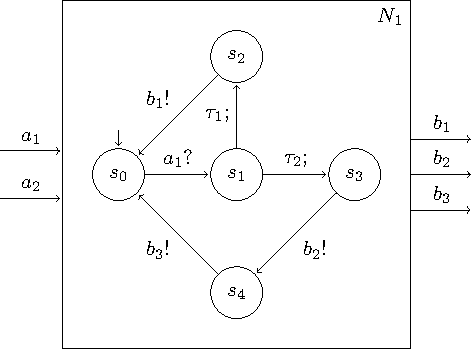
\includegraphics[width=8cm]{fig/sia.pdf}
    \CaptionFigSpace
    \caption{An example of a process $N_1$ where \gls{sia} $\descSIA{N}_1$ describes the interaction protocol of $N_1$.}
    \label{fig_sia}
    \BotFigSpace
\end{figure}
%------------------------------------------------------------------

Now, with a model to describe the interaction protocol of a process in a \gls{pnsc} I need to take a closer lock on how \glspl{sia} interact with each other.

%------------------------------------------------------------------------------
\subsection{Interaction of SIAs}
\label{sect_sia_interaction}
I use \glspl{sia} to describe the interaction protocol of processes in order to understand how processes interact with each other.
The idea is to perform a binary composition of two \glspl{sia}, each describing the protocol of a process.
% , perform an analysis on the composition and then further compose it with another \gls{sia}, describing another process of the \gls{pnsc}.
% This will be repeated until all processes of the \gls{pnsc} are included in the composition.
The formal method of the composition is described later in \Sect{\ref{sect_sia_composition}}.
In this section I describe how two \glspl{sia} $\descSIA{M}$ and $\descSIA{N}$ interact with each other and in particular how the actions of each particular \gls{sia} are controlled.

Input and output ports of a process define the interface of the process to its environment.
Input and output actions of a \gls{sia}, describing the protocol of this process, define how the process behaviour is interacting with the environment.
Shared actions represent the actual transmissions of messages from one process to another while shared ports represent the synchronous channels, spawned between processes.
Open actions represent the ability of a process to communicate with its environment via ports where the corresponding communication partner is not (yet) known.

In order to understand how a \gls{sia} reaches a state that is permanently blocking we have to understand how actions are controlled in more detail.
To do this I will first discuss the control of shared input and output actions.
For this purpose let's consider the example in \Fig{\ref{fig_sia_control_shared}}.
The two processes $M_1$ and $N_2$ share the ports $a$ and $b$ and their corresponding \glspl{sia} $\descSIA{M}_1$ and $\descSIA{N}_2$ share the action $a$.
The output action $b$ of \gls{sia} $\descSIA{N}_2$ is ignored.
%------------------------------------------------------------------
\begin{figure}[bht]
    \TopFigSpace
    \centering
    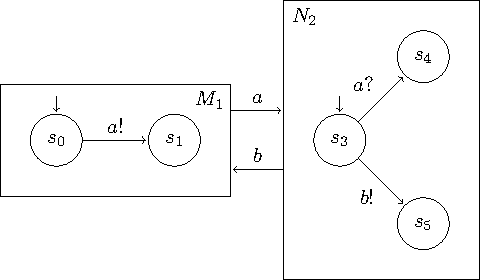
\includegraphics[width=8cm]{fig/sia_control_shared.pdf}
    \CaptionFigSpace
    \caption{A simple example of two processes $M_1$ and $N_2$ with their corresponding \glspl{sia} $\descSIA{M}_1$ and $\descSIA{N}_2$ connected by the channels $a$ and $b$.
    However, only action $a$ is shared.}
    \label{fig_sia_control_shared}
    \BotFigSpace
\end{figure}
%------------------------------------------------------------------

Initially, both \glspl{sia} $\descSIA{M}_1$ and $\descSIA{N}_2$ are in their initial state $s_0$  and $s_3$, respectively.
From both of these states action $a$ is enabled.
Additionally, action $b$ is enabled in state $s_3 \in S_{\descSIA{N}_2}$.
Hence, in state $s_3$ two transitions are possible.
However, as the output action $b$ will never be able to be served by $N_2$'s environment (\gls{sia} $\descSIA{M}_1$ in this case) because no matching input action is available, the transition $\langle s_3, b, s_5 \rangle$ will never be possible with the given environment $\descSIA{M}_1$.
Therefore, from their respective initial state $s_0$ and $s_3$, \glspl{sia} $\descSIA{M}_1$ and $\descSIA{N}_2$ transition to state $s_1$ and $s_4$, synchronized by the label $a$.
The decision in state $s_3 \in S_{\descSIA{N}_2}$ is imposed by the environment $\descSIA{M}_1$.

Let's now study the control of open actions.
Open actions are either of direction input or output, hence, blocking and non-autonomous.
However, in contrast to shared actions, with open actions the environment is not (yet) known.
Hence, an assumption has to be made whether the environment will eventually provide the corresponding counter parts of the open actions.
The goal of describing the protocol behaviour of processes with the help of \gls{sia} is to check all possible interaction behaviour in order to guarantee liveness.
Hence, I will assume a \emph{helpful} environment that is always providing open actions.
This guarantees that potential permanent blocking states, that are only reachable through open actions, will still be considered.
During the incremental composition of \glspl{sia}, open actions will eventually become shared actions and will then be considered where the environment is known.
Therefore, potential permanent blocking states caused by such actions will be detected at this later stage.

Note that open actions are, like shared actions, blocking and non-autonomous but because a helpful environment is assumed they will never block and will always be served.
Hence, open actions will always trigger the corresponding transitions in a \gls{sia}.
Such an example is illustrated in \Fig{\ref{fig_sia_control_open}} where two processes $M_1$ and $N_3$ are connected by the shared ports $a$ and $b$.
The interaction protocol of process $M_1$ is described by \gls{sia} $\descSIA{M}_1$.
Process $N_3$ has additional ports $d$ and $e$ which are not connected and its interaction protocol is described by \gls{sia} $\descSIA{N}_3$.
\Glspl{sia} $\descSIA{M}_1$ and $\descSIA{N}_3$ share the action $a$.
%------------------------------------------------------------------
\begin{figure}[bht]
    \TopFigSpace
    \centering
    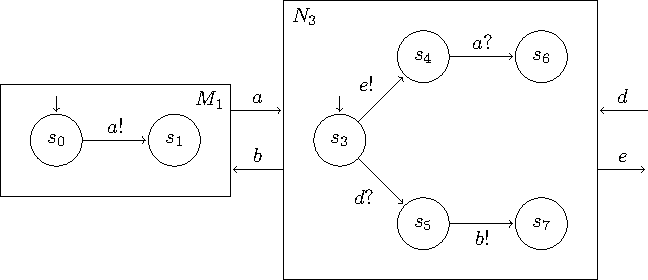
\includegraphics[width=11cm]{fig/sia_control_open.pdf}
    \CaptionFigSpace
    \caption{An example of a \gls{pnsc} where the \gls{sia} $\descSIA{N}_3$ of process $N_3$ has the open actions $d$ and $e$.}
    \label{fig_sia_control_open}
    \BotFigSpace
\end{figure}
%------------------------------------------------------------------

While \gls{sia} $\descSIA{M}_1$ resides in its initial state $s_0$, \gls{sia} $\descSIA{N}_3$ starts in state $s_3$ and can transition to either state $s_4$ or $s_5$ triggered by the open action $e$ or $d$, respectively.
As open actions are assumed to always be served by the environment, $\descSIA{N}_3$ can reach either of the states $s_4$ and $s_5$ while \gls{sia} $\descSIA{M}_1$ is blocked in state $s_0$.
With \gls{sia} $\descSIA{N}_3$ in state $s_4$, $\descSIA{M}_1$ and $\descSIA{N}_3$ synchronise on the shared action $a$ and transition to their respective state $s_1$ and $s_6$.
Because the action $b \in \mathcal{A}_{\descSIA{N}_3}$ is ignored, $\descSIA{N}_3$ cannot perform any further transition from state $s_5$ to state $s_7$.
Note that the decision at state $s_3 \in S_{\descSIA{N}_3}$ depends on a currently unknown environment.
At a later stage, a new process, interaction with its environment via ports $d$ and $e$, might be added to the \gls{pnsc}.
By this, the system will gain knowledge of the environment, with respect to ports $d$ and $e$ and consequently, the corresponding actions of the respective \gls{sia} will be turned into shared actions.

As established in the previous section, internal actions are controlled only by the process itself and not by the environment.
Hence, internal actions are independent of interactions and do trigger transitions autonomously.
The \gls{pnsc} illustrated in \Fig{\ref{fig_sia_control_internal}} shows the two interacting processes $M_1$ and $N_4$.
The interaction protocol of process $N_4$ includes transitions that are triggered by the internal actions $\tau_1$ and $\tau_2$.
%------------------------------------------------------------------
\begin{figure}[bht]
    \TopFigSpace
    \centering
    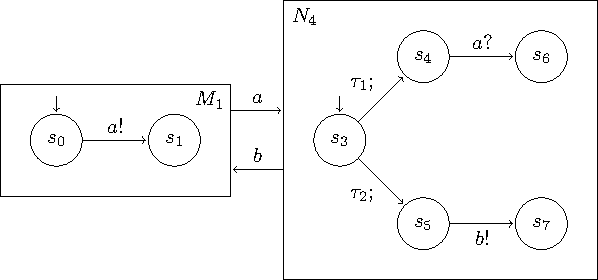
\includegraphics[width=10cm]{fig/sia_control_internal.pdf}
    \CaptionFigSpace
    \caption{An example of a \gls{pnsc} where the \gls{sia} $\descSIA{N}_4$ of process $N_4$ has the internal actions $\tau_1$ and $\tau_2$.}
    \label{fig_sia_control_internal}
    \BotFigSpace
\end{figure}
%------------------------------------------------------------------

While \gls{sia} $\descSIA{M}_1$ temporarily blocks in its initial state $s_0$, \gls{sia} $\descSIA{N}_4$ starts in state $s_3$ and can transition to either state $s_4$ or $s_5$.
The transitions are triggered by the internal actions $\tau_1$ and $\tau_2$, respectively.
In contrast to the example of \Fig{\ref{fig_sia_control_open}} where open actions are triggering the transitions, here the transitions are independent of the environment.
The choice at state $s_3 \in S_{\descSIA{N}_4}$ is unknown to the system because internal actions are hidden.

In \Fig{\ref{fig_sia_control_internal}}, the states $s_5 \in S_{\descSIA{N}_4}$ and $s_0 \in S_{\descSIA{M}_1}$ are permanent blocking states:
With both \glspl{sia} $\descSIA{M}_1$ and $\descSIA{N}_4$ starting in their respective initial state $s_0$ and $s_3$, an autonomous choice of process $N_4$ may lead to an internal transition of $\descSIA{N}_4$ to state $s_5$.
Because action $b \in \mathcal{A}_{\descSIA{N}_4}^O$ is ignored, a further transition from state $s_5$ will never be possible.
Hence, \gls{sia} $\descSIA{N}_4$ is blocking indefinitely in state $s_5$.
At the same time \gls{sia} $\descSIA{M}_1$ is still blocking in state $s_0$ and waits for \gls{sia} $\descSIA{N}_4$ to reach state $s_4$ in order to synchronize on shared action $a$.
In the current situation, this can never happen because \gls{sia} $\descSIA{N}_4$ is indefinitely blocking in state $s_5$ and therefore \gls{sia} $\descSIA{M}_1$ is indefinitely blocking in state $s_0$.

In contrast to the example with internal action (as depicted in \Fig{\ref{fig_sia_control_internal}}), the example with open actions (as depicted in \Fig{\ref{fig_sia_control_open}}) has permanent blocking states, only if the environment provides an action $d$.
This is because in \Fig{\ref{fig_sia_control_open}} the environment with respect to actions $d$ and $e$ might become known at a later stage and action $d$ might be ignored, the transition $\langle s_3, d, s_5 \rangle$ would not be possible and hence the permanent blocking state $s_5$ would never be reachable.
Consequently, \gls{sia} $\descSIA{M}_1$ might never be permanently blocked in state $s_0$.

Up to this point, this chapter gave an informal understanding what permanent blocking means.
\Chap{\ref{chap_block}} will provide a formal definition of permanent blocking states by analysing a composed system, as defined in \Sect{\ref{sect_sia_composition}}.

As an example of a composition, let's consider the \gls{pnsc} depicted in \Fig{\ref{fig_sia_ex}} where two processes $M_2$ and $N_4$ share the ports $a$ and $b$ and process $M_2$ has an unconnected port $c$.
%------------------------------------------------------------------
\begin{figure}[bht]
    \TopFigSpace
    \centering
    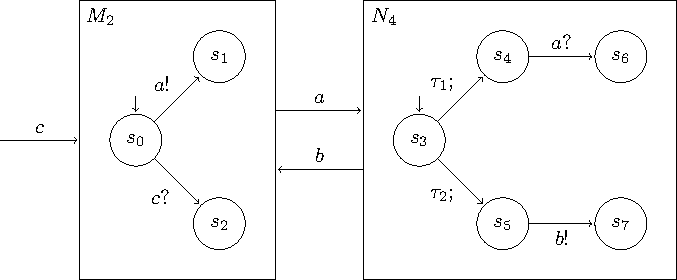
\includegraphics[width=11cm]{fig/sia_ex.pdf}
    \CaptionFigSpace
    % \caption{An example of a \gls{pnsc} with \glspl{sia} containing open actions, shared actions, ignored actions and internal must actions.}
    \caption{An example of a \gls{pnsc} with \glspl{sia} containing open actions, shared actions, ignored actions and internal actions.}
    \label{fig_sia_ex}
    \BotFigSpace
\end{figure}
%------------------------------------------------------------------
By folding their corresponding \glspl{sia} $\descSIA{M}_2$ and $\descSIA{N}_4$ into the resulting \gls{sia} $\descSIA{\mathit{M}_2\mathit{N}_4}$, a new composed process, I call it $\mathit{M}_2\mathit{N}_4$ in this example, is created.
The composed process $\mathit{M}_2\mathit{N}_4$ with its corresponding \gls{sia} $\descSIA{\mathit{M}_2\mathit{N}_4}$ is depicted in \Fig{\ref{fig_sia_ex_fold}}.
All unreachable states of \gls{sia} $\descSIA{\mathit{M}_2\mathit{N}_4}$ have been removed for the sake of readability.
%------------------------------------------------------------------
\begin{figure}[bht]
    \TopFigSpace
    \centering
    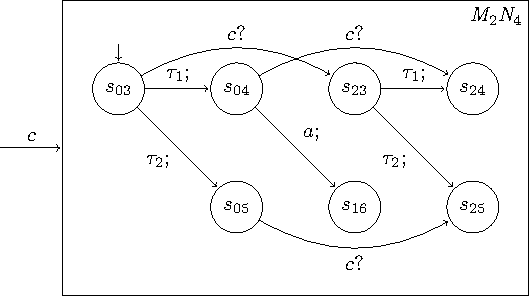
\includegraphics[width=9cm]{fig/sia_ex_fold.pdf}
    \CaptionFigSpace
    \caption{The composed process $\mathit{M}_2\mathit{N}_4$ with its composed \gls{sia} $\descSIA{\mathit{M}_2\mathit{N}_4}$ as a result of the composition of the system depicted in \Fig{\ref{fig_sia_ex}}.}
    \label{fig_sia_ex_fold}
    \BotFigSpace
\end{figure}
%------------------------------------------------------------------

The only remaining port of $\mathit{M}_2\mathit{N}_4$ is the unconnected port $c$ which relates to the open action $c \in \mathcal{A}_{\descSIA{\mathit{M}_2\mathit{N}_4}}^I$, triggering the transitions $\langle s_{03}, c, s_{23} \rangle$, $\langle s_{04}, c, s_{24} \rangle$, and $\langle s_{05}, c, s_{25} \rangle$.
Note that all transitions triggered by action $c \in \mathcal{A}_{\descSIA{\mathit{M}_2\mathit{N}_4}}^I$ change only the part of the state corresponding to the \gls{sia} $\descSIA{M}_2$.
The reason for this is that it is not possible to reach $s_{06}$ because $\descSIA{M}_2$ must transition to state $s_1$ in order to synchronize on action $a$.
State $s_{07}$ cannot be reached because action $b \in \mathcal{A}_{\descSIA{N}_4}^O$ is ignored.
With similar reasoning, I identify the internal actions $\tau_1$ and $\tau_2$ that originate from \gls{sia} $\descSIA{N}_4$.
The shared actions $a$ of the \glspl{sia} $\descSIA{M}_2$ and $\descSIA{N}_4$ are turned into the internal action $a \in \mathcal{A}_{\descSIA{\mathit{M}_2\mathit{N}_4}}^H$, triggering the transition $\langle s_{04}, a, s_{16} \rangle$.

%==============================================================================
\section{Modelling a Crossroad with SIAs}
\label{sect_ecm_example}
In this section I will apply the \gls{sia} model on the crossroad example described in \Fig{\ref{fig_cross_proc_dl}}.
The interaction behaviour of the processes $P_{\mathit{NW}}$, $P_{\mathit{NE}}$, $P_{\mathit{SE}}$, and $P_{\mathit{SW}}$ are modelled with the \glspl{sia} $\descSIA{P}_{\mathit{NW}}$, $\descSIA{P}_{\mathit{NE}}$, $\descSIA{P}_{\mathit{SE}}$, and $\descSIA{P}_{\mathit{SW}}$, respectively, as depicted in \Fig{\ref{fig_cross_proc_sia_dl}}.
%------------------------------------------------------------------
\begin{figure}[bht]
    \TopFigSpace
    \centering
    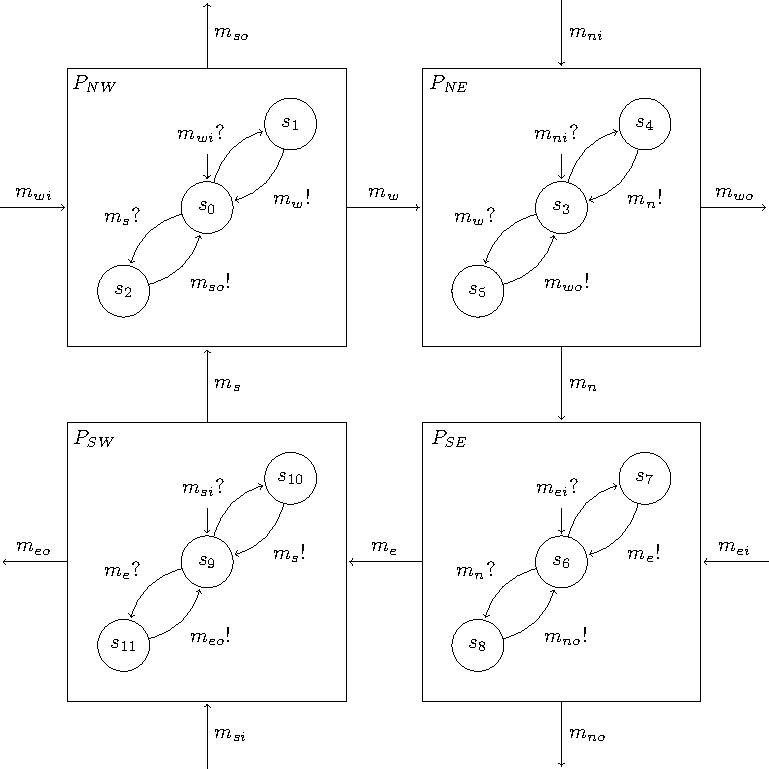
\includegraphics[width=12cm]{fig/cross_proc_sia_dl.pdf}
    \CaptionFigSpace
    \caption{A \gls{pnsc} model of \Fig{\ref{fig_cross_proc_dl}} extended by the corresponding \glspl{sia} of each process.
        Due to the symmetry of the model, the system can potentially reach a permanent blocking state --- a deadlock, involving all four processes.}
    \label{fig_cross_proc_sia_dl}
    \BotFigSpace
\end{figure}
%------------------------------------------------------------------
I will only explain the rationale behind the system behaviour with respect to the lane arriving from the West and going to the East ($m_{wi}$, $m_{w}$, $m_{wo}$) but as each \gls{sia} in this example is modelled in a similar fashion the explanation is applicable for all of the lanes.
At its initial state $s_0$ \gls{sia} $\descSIA{P}_{\mathit{NW}}$ is either triggered by the input action $m_{wi}$ or $m_s$.
Those actions correspond to allocating a space on the intersection for a car as explained in \Sect{\ref{sect_ecm_pnsc}}.
By triggering transition $\langle s_0, m_{wi}, s_1 \rangle$ the space $\mathit{NW}$ is allocated for the car arriving from the West.
The request for space $\mathit{NE}$ corresponds to the transition $\langle s_1, m_w, s_0 \rangle$.
The action $m_w$ is shared with \gls{sia} $\descSIA{P}_{\mathit{NE}}$, hence, the transition $\langle s_1, m_w, s_0 \rangle$ can only be triggered if $\descSIA{P}_{\mathit{NE}}$ is in its initial state $s_{3}$.
Triggered by the input action $m_w$, \gls{sia} $\descSIA{P}_{\mathit{NE}}$ performs the transition $\langle s_3, m_w, s_5 \rangle$ to allocate the space $\mathit{NE}$ to the car arriving from the West.
By performing transition $\langle s_5, m_{wo}, s_0 \rangle$, triggered by the output action $m_{wo}$, the car crosses the intersection and the spaces $\mathit{NW}$ and $\mathit{NE}$ are released.

The folding operation, described in \Sect{\ref{sect_sia_composition}}, is applied incrementally on the model such that the resulting \gls{sia} $\descSIA{P}_{res} = \descSIA{P}_{\mathit{NW}} \otimes \descSIA{P}_{\mathit{NE}} \otimes \descSIA{P}_{\mathit{SE}} \otimes \descSIA{P}_{\mathit{SW}}$ is produced.
By doing this we observe that the model is not free of permanent blocking.
The \gls{sia} $\descSIA{P}_{res}$ is depicted in \Fig{\ref{fig_cross_sia_dl}}\footnote{Produced with https://github.com/moiri/streamix-ifa} where a node, depicted as a black square, represents a state where no further progress is possible.
%------------------------------------------------------------------
\begin{figure}[bht]
    \TopFigSpace
    \centering
    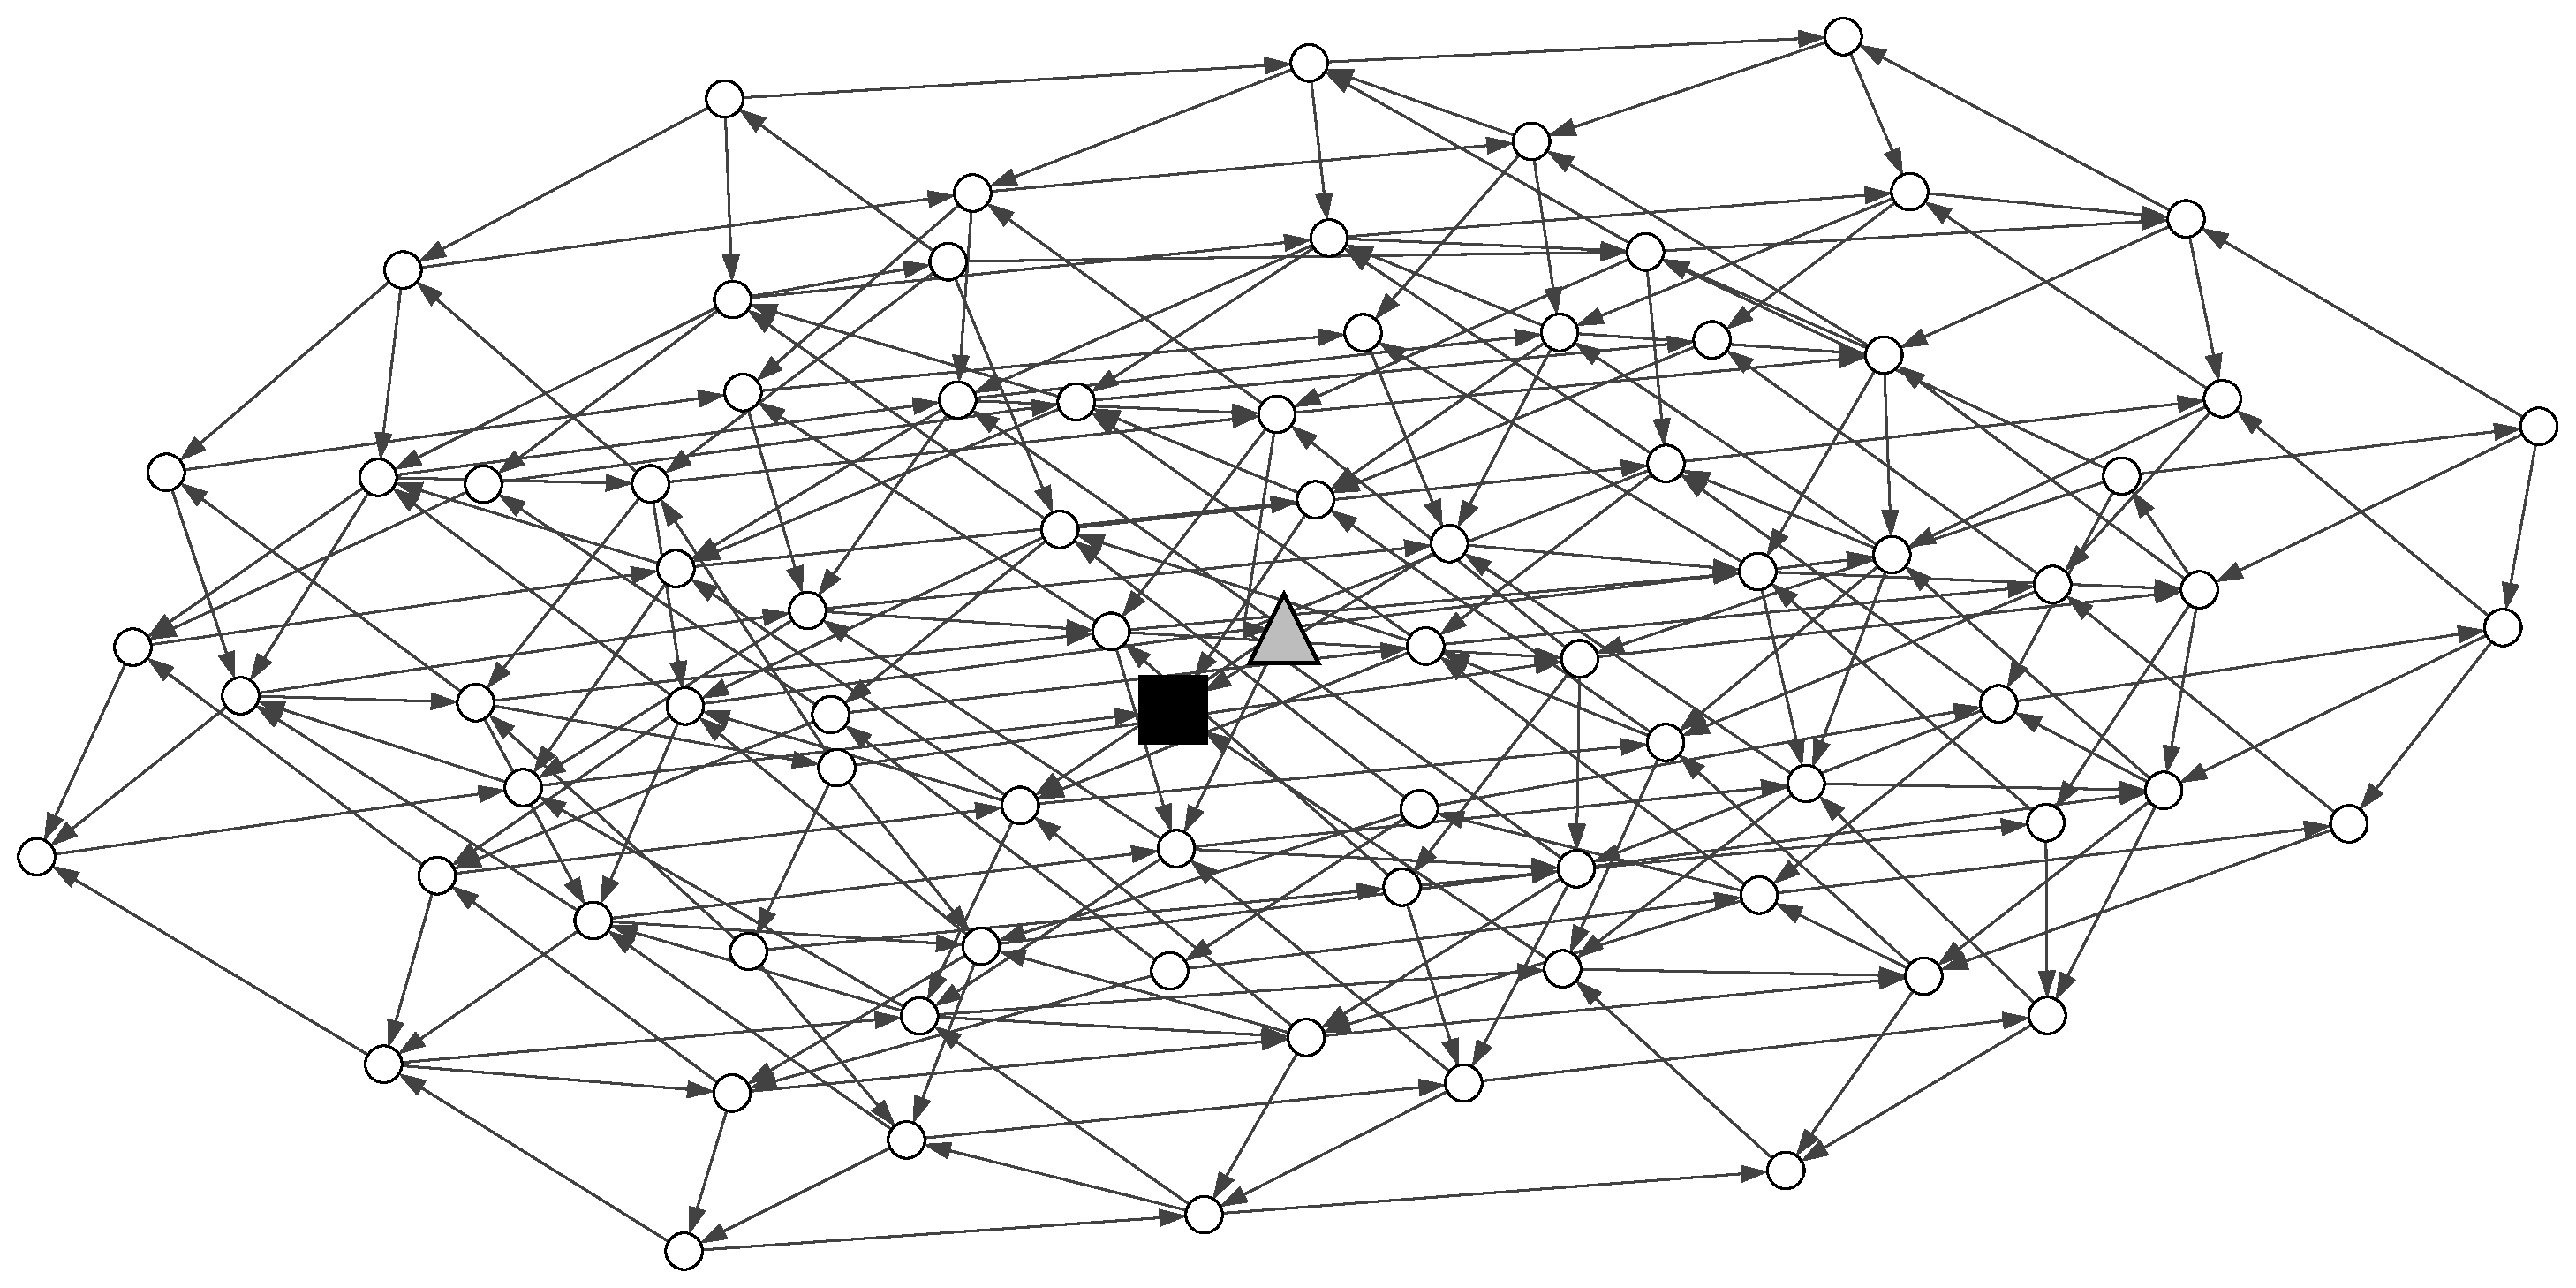
\includegraphics[width=10cm]{fig/cross_sia_dl.pdf}
    \CaptionFigSpace
    \caption{The graph representing the \gls{sia} $\descSIA{P}_{res}$.
        It consists of 80 states and 248 transitions.
        The black square node represents a state where no further transitions are possible and the grey triangle node represents the initial state.}
    \label{fig_cross_sia_dl}
    \BotFigSpace
\end{figure}
%------------------------------------------------------------------
The resulting \gls{sia} $\descSIA{P}_{res}$ of this system is already quite complex.
On the one hand this is due to the exponential growth of the state space.
There exist solutions to prevent state space explosion in \glspl{lts} (\eg~\cite{groote1996}) but I will not discuss this further in this dissertation and postpone the analysis of how such a method can be applied to the here presented model to future work.
On the other hand, the crossroad example has several open ports which causes the \gls{sia} $\descSIA{P}_{res}$ to describe every possible combination of cars, arriving and departing in a different order.
Connecting producer processes to the open ports can serve to impose an order on how cars arrive and depart from the intersection and reduce the system complexity.

As mentioned in \Sect{\ref{sect_background_comp}}, this crossroad situation can lead to a deadlock.
This is indicated by the state represented as a black square in \Fig{\ref{fig_cross_sia_dl}} where no further transitions are possible.
While an imposed order of departing cars can always cause potential permanent blocking by placing the system in a hostile environment (\eg a congestion on a lane after the intersection which prevents cars from freeing space on the intersection), the problem with this system is that the system can be stuck in a permanent blocking state even under the assumption that the open output actions $m_{wo}$, $m_{no}$, $m_{eo}$, and $m_{so}$ can always be served.
A simple example where a deadlock situation occurs is when allocating one space for each car on their respective lane.
This is illustrated by \Fig{\ref{fig_cross_sync_b}}.
The system is in a deadlock state because each \gls{sia} $\descSIA{P}_{\mathit{NW}}$, $\descSIA{P}_{\mathit{NE}}$, $\descSIA{P}_{\mathit{SE}}$, and $\descSIA{P}_{\mathit{SW}}$ synchronized on its respective input action $m_{wi}$, $m_{ni}$, $m_{ei}$, and $m_{si}$ and is permanently blocked in its respective state $s_1$, $s_4$, $s_7$, and $s_{10}$.

The fact that the model is not free of permanent blocking only means that there is the possibility of permanent blocking.
For example, let's assume that on each lane a car arrives and departs before another car arrives on any other lane.
%------------------------------------------------------------------
\begin{figure}[bht]
    \TopFigSpace
    \centering
    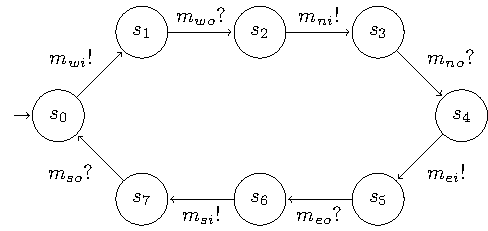
\includegraphics[width=7cm]{fig/cross_simple_env.pdf}
    \CaptionFigSpace
    \caption{An example of an environment $\descSIA{P}_{env}$ for the \gls{pnsc} of \Fig{\ref{fig_cross_proc_sia_dl}}.}
    \label{fig_cross_simple_env}
    \BotFigSpace
\end{figure}
%------------------------------------------------------------------
This is modelled by a \gls{sia} (representing the environment) $\descSIA{P}_{env}$ as depicted in \Fig{\ref{fig_cross_simple_env}}.
% We represent this as a list of actions: [$m_{wi}!$, $m_{wo}?$, $m_{ni}!$, $m_{no}?$, $m_{ei}!$, $m_{eo}?$, $m_{si}!$, $m_{so}?$].
% Every action in the list triggers a transition that leads to the next state in the circle.
% The first action in the list triggers the transition starting from the initial state and the last action in the list triggers the transition to the initial state, closing the circle.
Applying this environment to the system a trivial \gls{sia} $\descSIA{P}_{res} \otimes \descSIA{P}_{env}$ results, where in each state a transition is possible.
It is a single circle as depicted in \Fig{\ref{fig_cross_simple_res}}.
% [$m_{wi};$, $m_{w};$, $m_{wo};$, $m_{ni};$, $m_{n};$, $m_{no};$, $m_{ei};$, $m_{e};$, $m_{eo};$, $m_{si};$, $m_{s};$, $m_{so};$].
%------------------------------------------------------------------
\begin{figure}[bht]
    \TopFigSpace
    \centering
    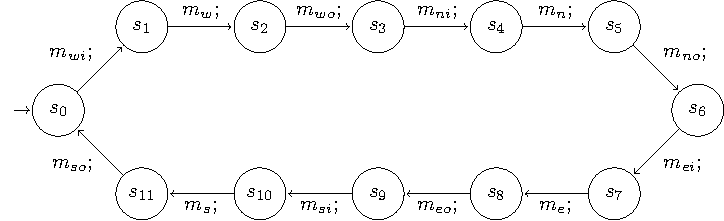
\includegraphics[width=10cm]{fig/cross_simple_res.pdf}
    \CaptionFigSpace
    \caption{The resulting \gls{sia} $\descSIA{P}_{res} \otimes \descSIA{P}_{env}$ when applying the environment $\descSIA{P}_{env}$ of \Fig{\ref{fig_cross_simple_env}} on the \gls{pnsc} $\descSIA{P}_{res}$ of \Fig{\ref{fig_cross_proc_sia_dl}}.}
    \label{fig_cross_simple_res}
    \BotFigSpace
\end{figure}
%------------------------------------------------------------------

In order to avoid the possibility of permanent blocking in the system of \Fig{\ref{fig_cross_proc_sia_dl}}, I have to change the topology of the \gls{pnsc} and, as a consequence, adapt the \glspl{sia} according to the changes.
The problem of the intersection is equivalent to the \emph{dining philosophers problem} with four philosophers and four forks.
Instead of sharing forks, as the philosophers are forced to do, the streams of cars have to share spaces.
The deadlock of the dining philosophers problem can be solved by imposing the rule that one philosopher starts by picking up the right fork while all others start by picking up the left fork.
Similarly, I break the circular wait in the crossroad example by letting process $P'_{\mathit{NW}}$ control the input flow from the West and the South and letting process $P'_{\mathit{SW}}$ control the output flow of the East and the South.
Consequently, the directions of the ports $m_s$ are changed such that process $P'_{\mathit{NW}}$ produces $m_s$ and $P'_{\mathit{SW}}$ consumes it (while before process $P_{\mathit{SW}}$ was producing $m_s$ and $P_{\mathit{NW}}$ consuming it).
The corresponding system is depicted in \Fig{\ref{fig_cross_proc_sia}}.
Note that only the processes $P'_{\mathit{NW}}$ and $P'_{\mathit{SW}}$ and their corresponding \glspl{sia} $\descSIA{P}'_{\mathit{NW}}$ and $\descSIA{P}'_{\mathit{SW}}$ are changed.
Processes $P_{\mathit{NE}}$ and $P_{\mathit{SE}}$ and their corresponding \glspl{sia} $\descSIA{P}_{\mathit{NE}}$ and $\descSIA{P}_{\mathit{SE}}$ stay the same as in \Fig{\ref{fig_cross_proc_sia_dl}}.
%------------------------------------------------------------------
\begin{figure}[bht]
    \TopFigSpace
    \centering
    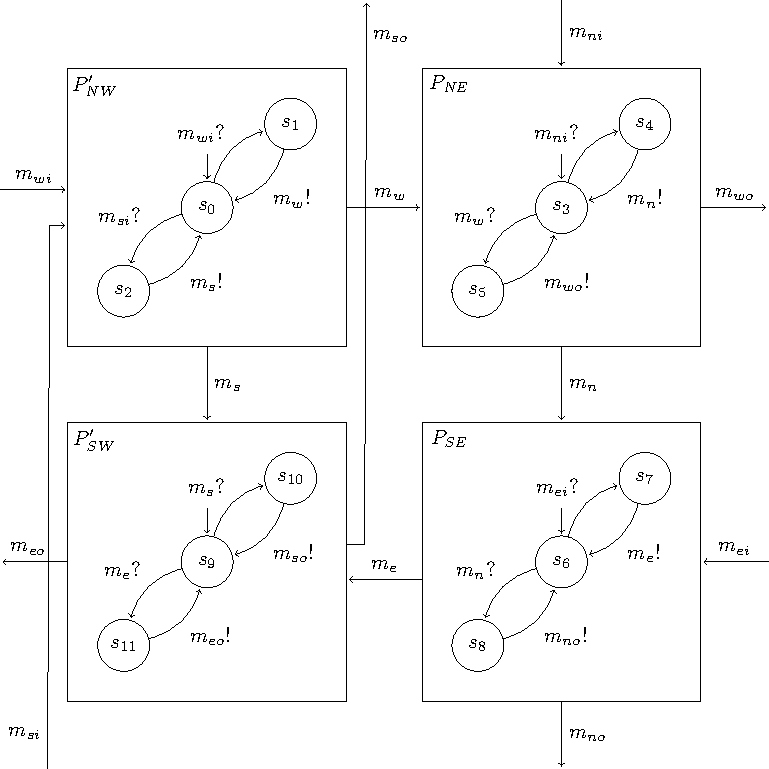
\includegraphics[width=12cm]{fig/cross_proc_sia.pdf}
    \CaptionFigSpace
    \caption{An adapted version of the crossroad model of \Fig{\ref{fig_cross_proc_sia_dl}} that breaks the symmetry and resolves the problem of permanent blocking.}
    \label{fig_cross_proc_sia}
    \BotFigSpace
\end{figure}
%------------------------------------------------------------------

% With this model the situation of \Fig{\ref{fig.cross.sync.b}} cannot occur because the actions $m_{si}$ and $m_{wi}$ cannot trigger two transitions simultaneous as they are both enabled in the same state $s_0$ of \gls{sia} $\descSIA{P}'_{\mathit{NW}}$.
With this model the situation of \Fig{\ref{fig_cross_sync_b}} cannot occur because the actions $m_{si}$ and $m_{wi}$ are both enabled in the same state $s_0$ of \gls{sia} $\descSIA{P}'_{\mathit{NW}}$ and only one of them can trigger a transition at a time.
By applying the folding operation $\otimes$ incrementally on the subsystems the resulting \gls{sia} $\descSIA{P}'_{res} = \descSIA{P}'_{\mathit{NW}} \otimes \descSIA{P}_{\mathit{NE}} \otimes \descSIA{P}_{\mathit{SE}} \otimes \descSIA{P}'_{\mathit{SW}}$, as depicted in \Fig{\ref{fig_cross_sia}}, is computed.
Here, from all states progress is possible.
%------------------------------------------------------------------
\begin{figure}[bht]
    \TopFigSpace
    \centering
    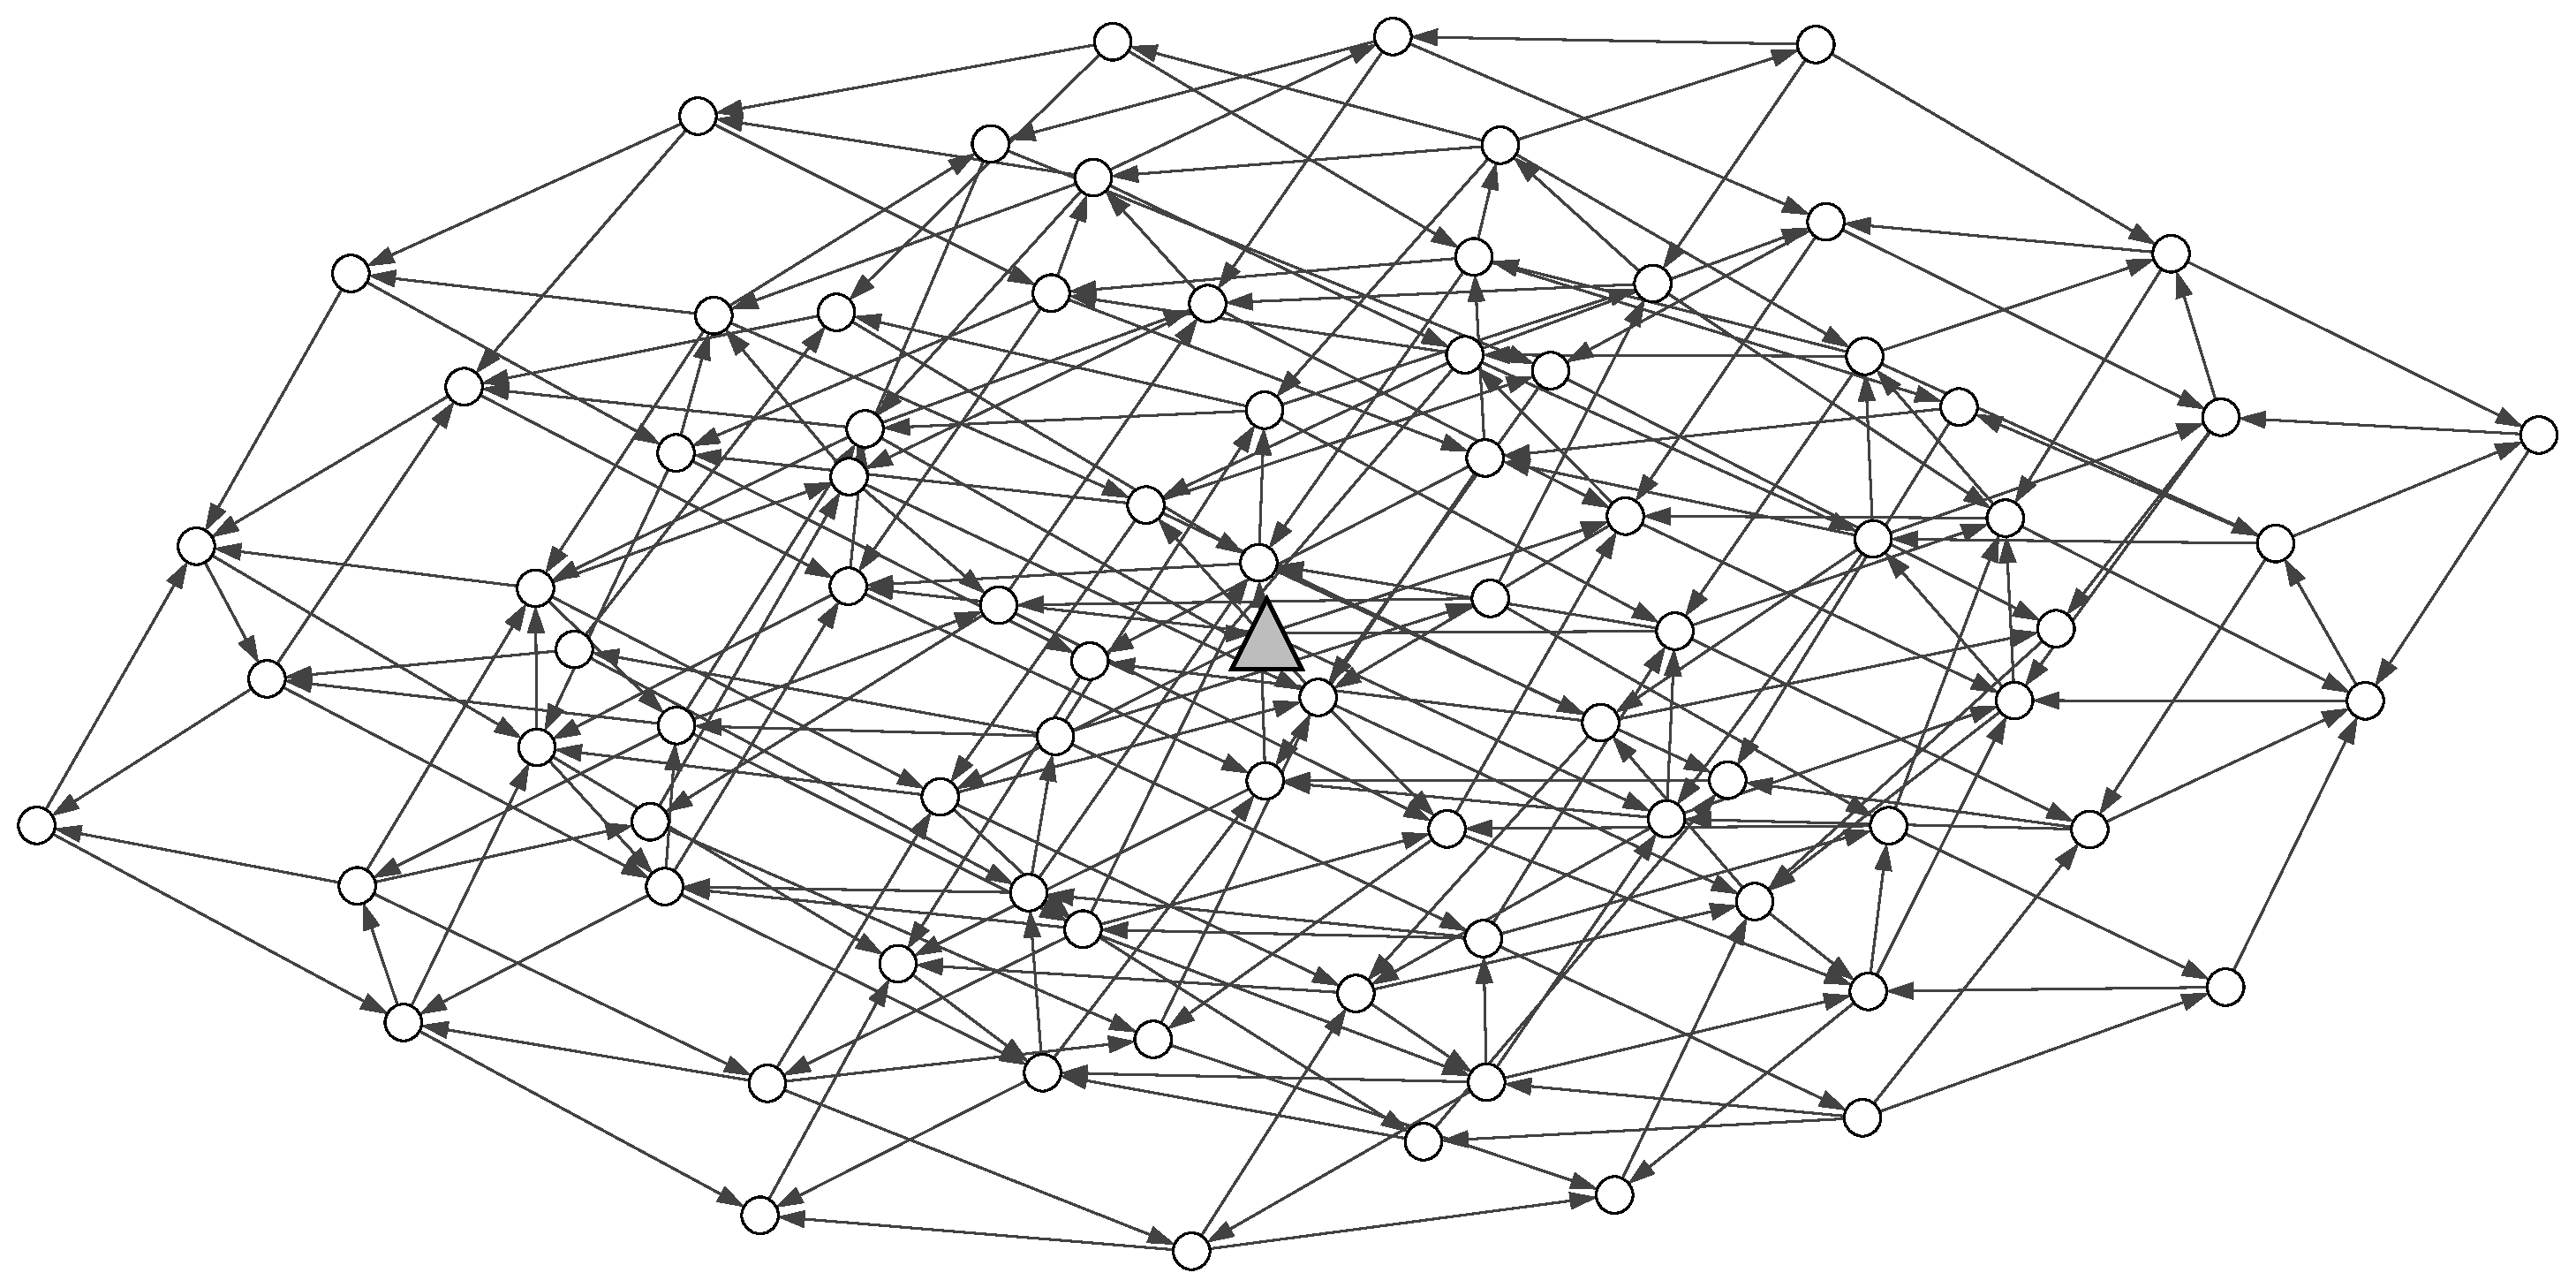
\includegraphics[width=10cm]{fig/cross_sia.pdf}
    \CaptionFigSpace
    \caption{The graph representing the \gls{sia} $\descSIA{P}'_{res}$.
        It consists of 81 states and 252 transitions.
        The grey triangle node represents the initial state of the system.}
    \label{fig_cross_sia}
    \BotFigSpace
\end{figure}
%------------------------------------------------------------------
As with the previous example (\Fig{\ref{fig_cross_proc_sia_dl}}), because the system is open it can be placed in a hostile environment where back pressure generated by a congestion would prevent cars from freeing occupied places and hence lead to a permanent blocking.
However, in contrast to the previous example, the redesigned system can cope with any input and will never block permanently.
% under the assumption that the open output actions are served in accordance to the input stream.

% The example of the crossing served to give an informal understanding of how a \gls{pnsc} can serve to detect problems of permanent blocking.
% In \Chap{\ref{chap_block}} I will describe a formal permanent blocking analysis that allows to identify local and global permanent blocking situations (including deadlocks).

%==============================================================================
\subsection{Streaming Network with Buffered Communication}
\label{sect_ecm_example_stream}
Up to this point I used a communication model based on synchronous communication.
In this section I describe how to model a streaming network with buffered communication which is asynchronous.

In general, a streaming network is a composition of computational components and directed channels.
Components consume and produce message tokens via input ports and output ports, respectively, at their interface.
The streaming network is spawned by a composition of components that are interlinked by channels.
A channel connects an input port with an output port and transmits message tokens via a \emph{\gls{fifo}} buffer.
Message tokens are produced sporadically by components while components are executed.
The execution of a component is triggered by message tokens arriving at the input ports of the component.
Every input port is an independent trigger of a component.
However, triggers become only active once the component is in the correct state to consume the message tokens at the corresponding input port.

If I map computational components and \gls{fifo} buffers to processes of a \gls{pnsc}, a streaming network can be described by the interaction model presented in this chapter.
The same as the interaction protocol of a process is described by a \gls{sia}, the order in which message tokens are consumed and produced by a computational component is described by a \gls{sia}.

%------------------------------------------------------------------
\begin{figure}[bht]
    \TopFigSpace
    \centering
    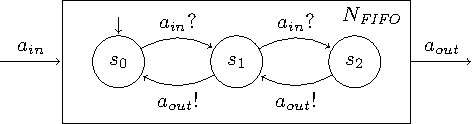
\includegraphics[width=9cm]{fig/sia_fifo.pdf}
    \CaptionFigSpace
    \caption{An example of a process $N_{FIFO}$ and its corresponding \gls{sia} $\descSIA{N}_{FIFO}$, modelling a \gls{fifo} buffer of length two with input $a_{in}$ and output $a_{out}$.}
    \label{fig_sia_fifo}
    \BotFigSpace
\end{figure}
%------------------------------------------------------------------
A \gls{fifo} buffer is modelled as a process with one input port and one output port.
The interaction protocol of a \gls{fifo} buffer is described by a \gls{sia} with an input and an output action that trigger one or more transitions.
\Fig{\ref{fig_sia_fifo}} depicts a process $P_{FIFO}$ and its corresponding \gls{sia} $\descSIA{P}_{FIFO}$, describing a \gls{fifo} buffer with two memory spaces.
In order to model a \gls{fifo} buffer with more memory spaces, the chain of states and transitions in the \gls{sia} is increased accordingly.

%------------------------------------------------------------------
\begin{figure}[bht]
    \TopFigSpace
    \centering
    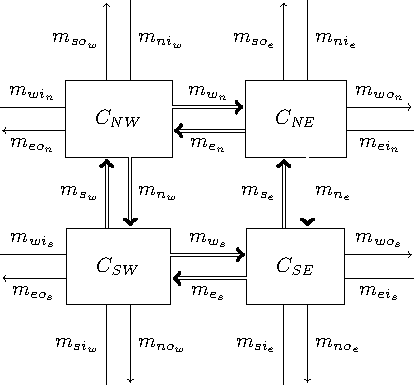
\includegraphics[width=9cm]{fig/cross_procs_dl.pdf}
    \CaptionFigSpace
    \caption{A \gls{pnsc} with four composed processes, each modelling an intersection as depicted in \Fig{\ref{fig_cross_proc_sia}}, interconnected by \gls{fifo} buffers (double-line arrows) forming a streaming network.}
    \label{fig_cross_procs_dl}
    \BotFigSpace
\end{figure}
%------------------------------------------------------------------
Applied on the crossroad example, multiple crossings can be connected as depicted in \Fig{\ref{fig_cross_procs_dl}}.
The four \glspl{pnsc} $C_{\mathit{NW}}$, $C_{\mathit{NE}}$, $C_{\mathit{SE}}$, and $C_{\mathit{SW}}$ each represent the assembly of processes modelling the deadlock-free crossroad behaviour (depicted in \Fig{\ref{fig_cross_proc_sia}}).
The composed \gls{sia} of \Fig{\ref{fig_cross_sia}} describes the interaction protocol of each of the computational components $C_{\mathit{NW}}$, $C_{\mathit{NE}}$, $C_{\mathit{SE}}$, and $C_{\mathit{SW}}$.
The double-line arrows represent \gls{fifo} channels that are connected to the corresponding input and output ports of the computational components.
The \gls{fifo} channels are modelled with processes that are similar to the process depicted in \Fig{\ref{fig_sia_fifo}}, but not necessarily of the same length.

Even though the system is composed of subsystems that are guaranteed to be free of permanent blocking, its is not guaranteed that the composed system is free of permanent blocking.
This is because of the back-pressure imposed on cars attempting to leave an intersection, caused by cars that are blocked in an intersection ahead.
The situation depicted in \Fig{\ref{fig_cross_buf}} is one example of a potential permanent blocking situation that can occur.
%------------------------------------------------------------------
\begin{figure}[bht]
    \TopFigSpace
    \centering
    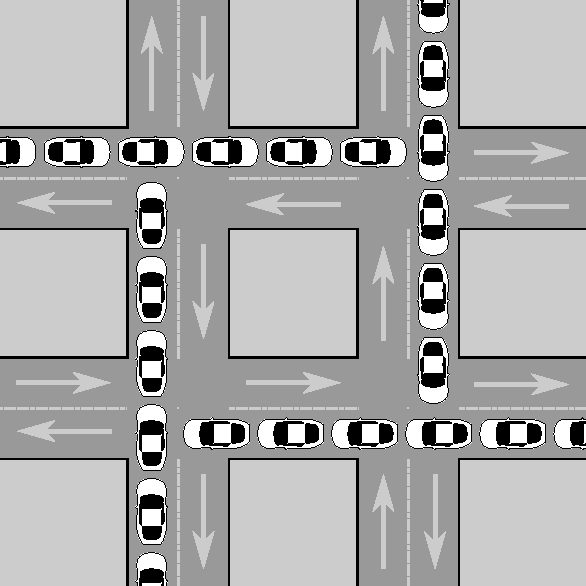
\includegraphics[width=7cm]{fig/cross_buf.pdf}
    \CaptionFigSpace
    \caption{A gridlock with four intersections. This system is modelled by a \gls{pnsc} in \Fig{\ref{fig_cross_procs_dl}}.}
    \label{fig_cross_buf}
    \BotFigSpace
\end{figure}
%------------------------------------------------------------------

%==============================================================================
\section{Chapter Summary}
\label{sect_ecm_summary}
In this chapter I introduced the \gls{pnsc} model.
It allows to describe networks of processes that are connected through synchronous channels.
In order to describe the interaction of a process with its environment I introduced \glspl{sia}.
A \gls{sia} is an automata-based model that describes the interaction protocol of a process where actions trigger transitions from one protocol state to another.
The model allows to compose processes and their corresponding \glspl{sia} in order to provide an abstract representation of the network.
This allows to build hierarchical networks and to reuse sub-networks as composed processes.
Due to the synchronous communication semantics of the channels, \glspl{sia} provide a rigorous language to describe the blocking behaviour of processes.

I used an example of a crossroad to illustrate the power of the model to analyse the interaction of processes.
I used the same example in a bigger context where each crossroad, as a composed process, is part of bigger system, modelled as a streaming application.
